%%%%%%%%%%%%%%%%%%%%%%%%%%%%%%%%%%%%%%%%%
% Beamer Presentation
% LaTeX Template
% Version 1.0 (10/11/12)
%
% This template has been downloaded from:
% http://www.LaTeXTemplates.com
%
% License:
% CC BY-NC-SA 3.0 (http://creativecommons.org/licenses/by-nc-sa/3.0/)
%
%%%%%%%%%%%%%%%%%%%%%%%%%%%%%%%%%%%%%%%%%

%----------------------------------------------------------------------------------------
%	PACKAGES AND THEMES
%----------------------------------------------------------------------------------------

\documentclass{beamer}

\mode<presentation> {

% The Beamer class comes with a number of default slide themes
% which change the colors and layouts of slides. Below this is a list
% of all the themes, uncomment each in turn to see what they look like.

%\usetheme{default}
%\usetheme{AnnArbor}
%\usetheme{Antibes}
%\usetheme{Bergen}
%\usetheme{Berkeley}
%\usetheme{Berlin}
%\usetheme{Boadilla}
%\usetheme{CambridgeUS}
%\usetheme{Copenhagen}
%\usetheme{Darmstadt}
%\usetheme{Dresden}
%\usetheme{Frankfurt}
%\usetheme{Goettingen}
%\usetheme{Hannover}
%\usetheme{Ilmenau}
%\usetheme{JuanLesPins}
%\usetheme{Luebeck}
\usetheme{Madrid}
%\usetheme{Malmoe}
%\usetheme{Marburg}
%\usetheme{Montpellier}
%\usetheme{PaloAlto}
%\usetheme{Pittsburgh}
%\usetheme{Rochester}
%\usetheme{Singapore}
%\usetheme{Szeged}
%\usetheme{Warsaw}

% As well as themes, the Beamer class has a number of color themes
% for any slide theme. Uncomment each of these in turn to see how it
% changes the colors of your current slide theme.

%\usecolortheme{albatross}
%\usecolortheme{beaver}
%\usecolortheme{beetle}
%\usecolortheme{crane}
%\usecolortheme{dolphin}
%\usecolortheme{dove}
%\usecolortheme{fly}
%\usecolortheme{lily}
%\usecolortheme{orchid}
%\usecolortheme{rose}
%\usecolortheme{seagull}
%\usecolortheme{seahorse}
%\usecolortheme{whale}
%\usecolortheme{wolverine}

%\setbeamertemplate{footline} % To remove the footer line in all slides uncomment this line
%\setbeamertemplate{footline}[page number] % To replace the footer line in all slides with a simple slide count uncomment this line

%\setbeamertemplate{navigation symbols}{} % To remove the navigation symbols from the bottom of all slides uncomment this line
}

\usepackage{graphicx} % Allows including images
\usepackage{booktabs} % Allows the use of \toprule, \midrule and \bottomrule in tables
\usepackage{listings}
\usepackage[utf8x]{inputenc}
\def\lstlanguagefiles{lstlean.tex}
\lstset{language=lean}



%----------------------------------------------------------------------------------------
%	TITLE PAGE
%----------------------------------------------------------------------------------------

\title[Word problem in groups]{The word problem in one-relator groups} % The short title appears at the bottom of every slide, the full title is only on the title page

\author{Chris Hughes} % Your name
\institute[Imperial College London] % Your institution as it will appear on the bottom of every slide, may be shorthand to save space
{
Imperial College London \\ % Your institution for the title page
\medskip
}
\date{5th January 2021} % Date, can be changed to a custom date

\begin{document}

\lstset{language=lean}

\begin{frame}
\titlepage % Print the title page as the first slide
\end{frame}

\begin{frame}
\frametitle{The problem} % Table of contents slide, comment this block out to remove it

The one-relator tactic can prove an equality in a group given
one equality of group expressions. \newline

It is an implementation of an algorithm by Wilhem Magnus (1932). \newline

For example, \newline

Let $G$ be a group and let $a, b, c$ be elements of $G$.
\begin{equation*}
  \begin{aligned}
  \text{If } abab^2 = 1 \text{ then prove } ab=ba \\
  \text{If } ab = b^2 a \text{ then prove } a^2b = b^4 a^2
  \end{aligned}
\end{equation*}
\end{frame}

\begin{frame}
  \frametitle{A Story}
  I wrote this tactic. Once I wrote it, my supervisor Kevin Buzzard tweeted about it. \newline

  A bunch of people replied saying that there are better ways of solving this problem. \newline

  There are practical \textit{semidecision} procedures that solve the problem for more than one
  relation. \newline

\end{frame}


\begin{frame}
  \frametitle{Two Semidecision Procedures}
  Knuth Bendix is one well know algorithm that can be used as a semidecision procedure
  for multiple relations. \newline

  Kyle Miller (Berkeley) commented on twitter that he had another
  semidecision procedure for multiple relations. (It is on his website).
\end{frame}


\begin{frame}
  \frametitle{Semi Decision Procedures vs Decision Procedures}

  \textit{Semidecision} procedures terminates in a proof when the equality is true, but may not terminate
  when the goal is not provable. \newline

  \textit{Decision} procedures always terminate on whether the goal is provable or not.

\end{frame}

\begin{frame}
  Given a group $G$, and $a, b \in G$, if $ab=ba^2$ and $ba=ab^2$ then $a=1$. \newline

  There exists a group $G$, and $a, b \in G$, such that
    $ab=ba^2$ and $ba=ab^2$, but $a \ne 1$.
\end{frame}

\begin{frame}
  \frametitle{Knuth Bendix}
  Given a set of relations the Knuth Bendix algorithm finds a confluent rewriting system
  for those relations.

  E.g, given the equalities
  \begin{equation*}
     a^4 = 1, b^2 = 1, bab=a^3
  \end{equation*}
  Knuth Bendix generates the rewriting procedure
  \begin{equation*}
    \begin{aligned}
    aa^{-1} = 1 \\
    a^{-1}a = 1 \\
    b^2 = 1 \\
    a^{-2} = a^2 \\
    b^{-1} = b \\
    ba = a^{-1}b \\
    ba^{-1} = ab
    \end{aligned}
  \end{equation*}
Usually there is no such \textit{finite} rewriting procedure
\end{frame}


\begin{frame}
  \frametitle{Path Search Method}
    As an example consider the relation $abab^2 = 1$ and suppose we are trying to
    prove $ab = ba$. \newline

    First rearrange $ab=ba$ to the form $aba^{-1}b^{-1}=1$ \newline

    The relation $abab^2$ can be rearranged to a bunch of different equations,
    each with one letter on the lhs.
    \begin{equation*}
      \begin{aligned}
        a = b^{-2}a^{-1}b^{-1}, && a^{-1} = bab^2 \\
        b = a^{-1}b^{-2}a^{-1}, && b^{-1} = ab^2a \\
        a = b^{-1}a^{-1}b^{-2}, && a^{-1}=b^2ab \\
        b = a^{-1}b^{-1}a^{-1}b^{-1}, && b^{-1} = baba \\
        b = b^{-1}a^{-1}b^{-1}a^{-1}, && b^{-1} = abab \\
      \end{aligned}
    \end{equation*}
\end{frame}

\begin{frame}
  We generate the set of all words that can be reached from my starting node by
  applying one rewrite rule once,
  reduce the generated words, and add each generated word to a set of nodes $S$. \newline

  For example, applying the rewrite $a=b^{-2}a^{-1}b^{-1}$, we obtain the equality
  $\textcolor{red}{a}ba^{-1}b^{-1} = \textcolor{red}{b^{-2}a^{-1}b^{-1}}ba^{-1}b^{-1} =
  b^{-2}a^{-2}b^{-1}$. The word $b^{-2}a^{-2}b^{-1}$ is then added to $S$.
  \newline

  We then take the shortest word in $S$ and repeat the process,
  maintaining a list of seen words to avoid repeating any words.

\end{frame}

\begin{frame}
  \frametitle{Word Length}
  Cyclically reduce words at each stage
  \begin{equation*}
    aba^{-1}b^{-1}a^{-1}
  \end{equation*}
\end{frame}

\begin{frame}
  \frametitle{Word Length}
  Cyclically reduce words at each stage
  \begin{equation*}
    \color{red}ab\color{black}a^{-1}\color{red}b^{-1}a^{-1}
  \end{equation*}
\end{frame}

\begin{frame}
  \frametitle{Word Length}
  Cyclically reduce words at each stage
  \begin{equation*}
    \color{white}ab\color{black}a^{-1}\color{white}b^{-1}a^{-1}
  \end{equation*}
\end{frame}


\begin{frame}
  \frametitle{Tactic Outline}
  \begin{enumerate}
    \item Convert all hypotheses to the form $r_i = 1$, and the goal to the form $w = 1$
    \item Reify hypotheses $r_i$ and goal $w$ in the local context
      into a list of free group expressions.
    \item Search for a path using an efficient representation of the free group,
       whilst keeping track of enough information to retrace the path.
    \item Construct a Lean proof from the traced path.
  \end{enumerate}
\end{frame}

\begin{frame}{Keeping track of proofs}
  Given an old word $w$, such that $w$, a proof step is the following
  \begin{equation*}
    \begin{aligned}
      \text{Words } w_1 \text{ and } w_2 \text{, such that } w_1w_2 = w \\
      \text{A relation } r_i\text{ such that }r_i \approx 1 \\
      \text{Two words } a \text{ and } b \\
    \end{aligned}
  \end{equation*}
  If $w \approx 1$, then $a^{-1}w_1b^{-1}rbw_2a \approx 1$.
\end{frame}

\begin{frame}
  \frametitle{Proof}
  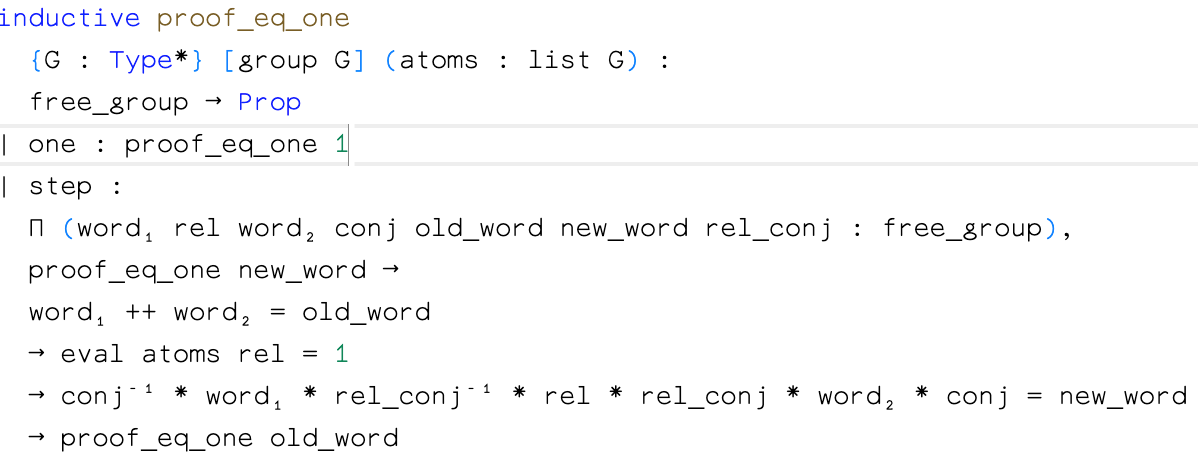
\includegraphics[width=\linewidth]{Screenshot.png}
\end{frame}

\begin{frame}[t]
  \frametitle{Comparison of Three Methods}
  \begin{columns}
    \begin{column}{0.33\textwidth}
      \centering{\textbf{Magnus' Method}}
      \begin{itemize}
        \item Decision procedure
        \item One relation
        \item Implemented in Lean
        \item Very complex (months of work to implement)
      \end{itemize}
    \end{column}
    \begin{column}{0.33\textwidth}
      \centering{\textbf{Path Search Method}}
      \begin{itemize}
        \item Semidecision Procedure
        \item Multiple relations
        \item Implemented in Lean
        \item Quite simple ($\sim$1 week to implement)
      \end{itemize}
    \end{column}
    \begin{column}{0.33\textwidth}
      \centering{\textbf{Knuth Bendix}}
      \begin{itemize}
        \item Semidecision Procedure
        \item Multiple relations
        \item Not implemented in Lean
        \item GAP, MAGMA have nonverified implementations
      \end{itemize}
    \end{column}
  \end{columns}
\end{frame}

\begin{frame}
  Demo
\end{frame}

% \begin{frame}
%   \frametitle{What I've Learnt}
%     Brute forcey methods work when there are a small number of hypotheses,
%     and the proof, if it exists, is not very long.

% \end{frame}

\begin{frame}
  \frametitle{What I've Learnt}
  \begin{itemize}
    \item Brute forcey methods work when there are a small number of hypotheses,
    and the proof, if it exists, is not very long.
    \item Often we don't really want a decision procedure, we only need
      a semidecision procedure.
  \end{itemize}
\end{frame}

\begin{frame}
  \frametitle{What I've Learnt}
    Brute forcey methods work when there are a small number of hypotheses,
    and the proof, if it exists, is not very long.
  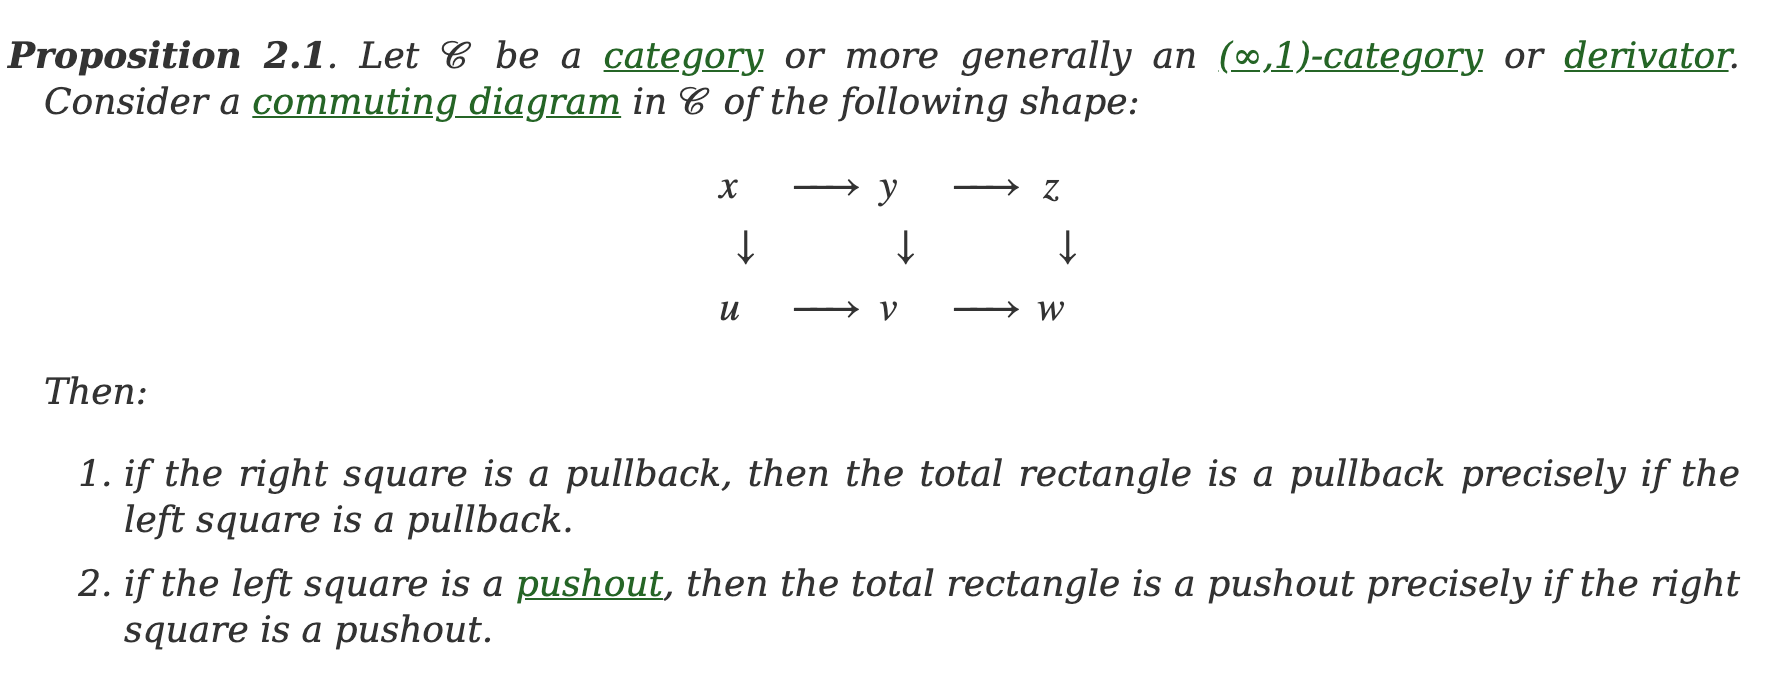
\includegraphics[width=\linewidth]{nlab.png}
  \textcolor{blue}{https://ncatlab.org/nlab/show/pasting+law+for+pullbacks}
\end{frame}



\begin{frame}
  \centering{Questions}
\end{frame}

\end{document}
